\documentclass[11pt,a4paper]{article}

\usepackage[spanish,es-nodecimaldot]{babel}
\usepackage[T1]{fontenc}
\usepackage[utf8]{inputenc}
\usepackage{lmodern}
\usepackage{geometry}
\usepackage{graphicx}
\usepackage{float}
\usepackage{hyperref}
\usepackage{enumitem}
\usepackage{booktabs}
\usepackage{tabularx}
\usepackage{longtable}
\usepackage{xurl}
\usepackage{amsmath}
\usepackage{listings}

\geometry{margin=2.5cm}
\hypersetup{colorlinks=true,linkcolor=black,urlcolor=blue,
    pdftitle={Análisis de tráfico DNS y exfiltración de datos},pdfauthor={Javier Siñuka}}
\graphicspath{{evidencias/}}
\lstset{basicstyle=\small\ttfamily,breaklines=true,columns=fullflexible,
    keepspaces=true,showstringspaces=false,frame=single}
\setlength{\emergencystretch}{2em}

\title{Análisis de tráfico DNS y exfiltración de datos}
\author{Javier Siñuka}
\date{20 de septiembre de 2026}

\begin{document}
\renewcommand{\tablename}{Tabla}
\maketitle

\section{Objetivo}

El objetivo fue observar cómo se resuelven nombres mediante DNS, identificar
la información transportada por Ethernet, IPv4, UDP y DNS, y comprobar cómo
un intercambio de consultas puede transportar datos que no forman parte de
una resolución de nombres convencional. Resolvimos las prácticas
\emph{Exploring DNS Traffic} (17.1.7) y \emph{Using Wireshark to Examine a UDP
DNS Capture} (10.2.7), y realizamos una transferencia controlada de un archivo
ficticio dentro de una red aislada.

Trabajamos con una VM Cisco existente. Conservamos las capturas originales,
los resultados de los comandos y las imágenes del escritorio de la VM. La
demostración permitió recuperar 1072 bytes tanto desde el receptor como desde
el PCAP. Finalmente, ejecutamos una detección basada en las características
de las consultas y la comparamos con una muestra de resolución normal.

\section{Conceptos utilizados}

DNS organiza nombres en una jerarquía y permite consultar registros asociados
con ellos. Un registro A contiene una dirección IPv4; AAAA, una IPv6; CNAME
indica un alias hacia otro nombre. El \emph{resolver} recibe la pregunta del
cliente y obtiene la respuesta desde su caché o consultando otros servidores.
En una resolución recursiva, el cliente solicita una respuesta final; el
resolver puede recorrer la jerarquía mediante consultas iterativas. Capturar
el enlace del cliente sólo muestra su intercambio con el resolver, no todos
los intercambios realizados después por éste~\cite{rfc1034}.

El mensaje DNS incluye un identificador de transacción de 16 bits, flags y
contadores de las secciones \emph{Questions}, \emph{Answers}, \emph{Authority}
y \emph{Additional}. El bit QR distingue consulta de respuesta; RD solicita
recursión y RA anuncia su disponibilidad. AA indica una respuesta autoritativa,
TC señala truncamiento y RCODE expresa el resultado. El TTL de cada registro
limita su permanencia en caché. Los nombres se transmiten como etiquetas;
cada etiqueta admite hasta 63 octetos y el nombre completo, en su codificación
de red, hasta 255~\cite{rfc1035}.

UDP transporta datagramas sin establecer previamente una conexión. Su
cabecera ocupa 8 bytes: cuatro campos de 16 bits correspondientes a puerto
origen, puerto destino, longitud y checksum. La longitud incluye cabecera y
datos. El checksum cubre cabecera, datos y un pseudoencabezado IP; no es una
firma criptográfica ni garantiza autenticidad~\cite{rfc768}. En una consulta
convencional, el cliente usa un puerto efímero y envía al puerto 53. La
respuesta invierte los extremos. El cliente relaciona ambos mensajes mediante
direcciones, puertos, identificador y pregunta.

DNS también utiliza TCP. Una respuesta UDP truncada puede requerir un nuevo
intento por TCP, y las implementaciones generales deben soportarlo. Por ello,
no sería correcto afirmar que DNS siempre funciona sobre UDP~\cite{rfc7766}.
EDNS permite anunciar capacidades, incluido un tamaño UDP mayor que el límite
histórico de 512 bytes~\cite{rfc6891}. En nuestras consultas con \texttt{dig}
usamos \texttt{+noedns} para obtener mensajes simples y comparables.

Wireshark permite examinar la lista de paquetes, el árbol de protocolos y los
bytes de la captura~\cite{wireshark}. La MAC identifica el siguiente destino
en el enlace local; la IP identifica el destino de la capa de red. Cuando
un servidor está fuera de la subred, se conserva su IP como destino, pero la
trama se entrega a la MAC del gateway. Si está directamente conectado, se
utiliza la MAC correspondiente a ese servidor o a su implementación virtual.

\section{Entorno y alcance de la ejecución}
\label{sec:entorno}

Antes de comenzar inspeccionamos el host Ubuntu 24.04.4 LTS. Encontramos
VirtualBox 7.2.14, Docker, Python 3.12.3, \texttt{tcpdump}, \texttt{dig},
\texttt{nslookup}, \texttt{host}, \texttt{xwd} y las herramientas de LaTeX.
Wireshark y tshark no estaban instalados en el host. No encontramos ejecutables
de QEMU, virsh, VMware ni Podman, ni el dispositivo \nolinkurl{/dev/kvm}.
Estas observaciones describen la inspección realizada; no prueban la ausencia
de cualquier instalación no registrada en las rutas habituales.

VirtualBox tenía registradas \emph{CyberOps Security Onion} y
\emph{Cybersecurity LabVM Worksation 20230210}, ambas apagadas. Iniciamos la
segunda, cuya descripción y pantalla de acceso incluyen el perfil SOC Analyst
para CyberOps Associate. En ella utilizamos la cuenta educativa
\texttt{analyst}, Ubuntu 22.04.1 LTS y Wireshark 3.6.7. No fue necesario
instalar software: \texttt{dumpcap}, \texttt{rawshark}, Python, \texttt{dig}
y \texttt{nslookup} ya estaban disponibles. El usuario pertenecía al grupo
\texttt{wireshark} y \texttt{dumpcap} tenía capacidades de captura.

Se utilizó, por tanto, la estación Cisco disponible con el perfil CyberOps,
no una instalación del host presentada como VM ni una copia supuesta de la
antigua imagen del DOCX. Conservamos el adaptador NAT preexistente. La práctica
10.2.7 describe un adaptador puente; ésta es una adaptación explícita, admitida
por la consigna general. Mantiene el análisis de Ethernet/IP/UDP/DNS sin
exponer una nueva máquina directamente a la LAN.

El host tenía la interfaz activa \texttt{wlp5s0}, IP \nolinkurl{192.168.1.163}
y gateway/resolver IPv4 \nolinkurl{192.168.1.1}. Esos valores no se mezclan con
los de las tablas de la práctica, que corresponden a la VM.

\begin{table}[H]
\centering
\caption{Configuración real de la estación utilizada; primera tabla del laboratorio 10.2.7.}
\label{tab:configuracion}
\begin{tabularx}{\textwidth}{lX}
\toprule
Descripción & Configuración observada \\
\midrule
Interfaz & \texttt{enp0s3}, adaptador NAT de VirtualBox \\
Dirección IP & \nolinkurl{10.0.2.15/24} \\
Dirección MAC & \texttt{08:00:27:55:44:07} \\
Gateway predeterminado & \nolinkurl{10.0.2.2} \\
DNS de \nolinkurl{/etc/resolv.conf} & \nolinkurl{127.0.0.53}, stub local de systemd-resolved \\
DNS efectivo del enlace & \nolinkurl{10.0.2.3}; también se anuncia
\texttt{fd17:625c:f037:2::3} \\
DNS consultado en el PCAP & \nolinkurl{10.0.2.3:53}, IPv4/UDP \\
Rango local de puertos efímeros & \texttt{32768--60999} \\
\bottomrule
\end{tabularx}
\end{table}

\begin{figure}[H]
\centering
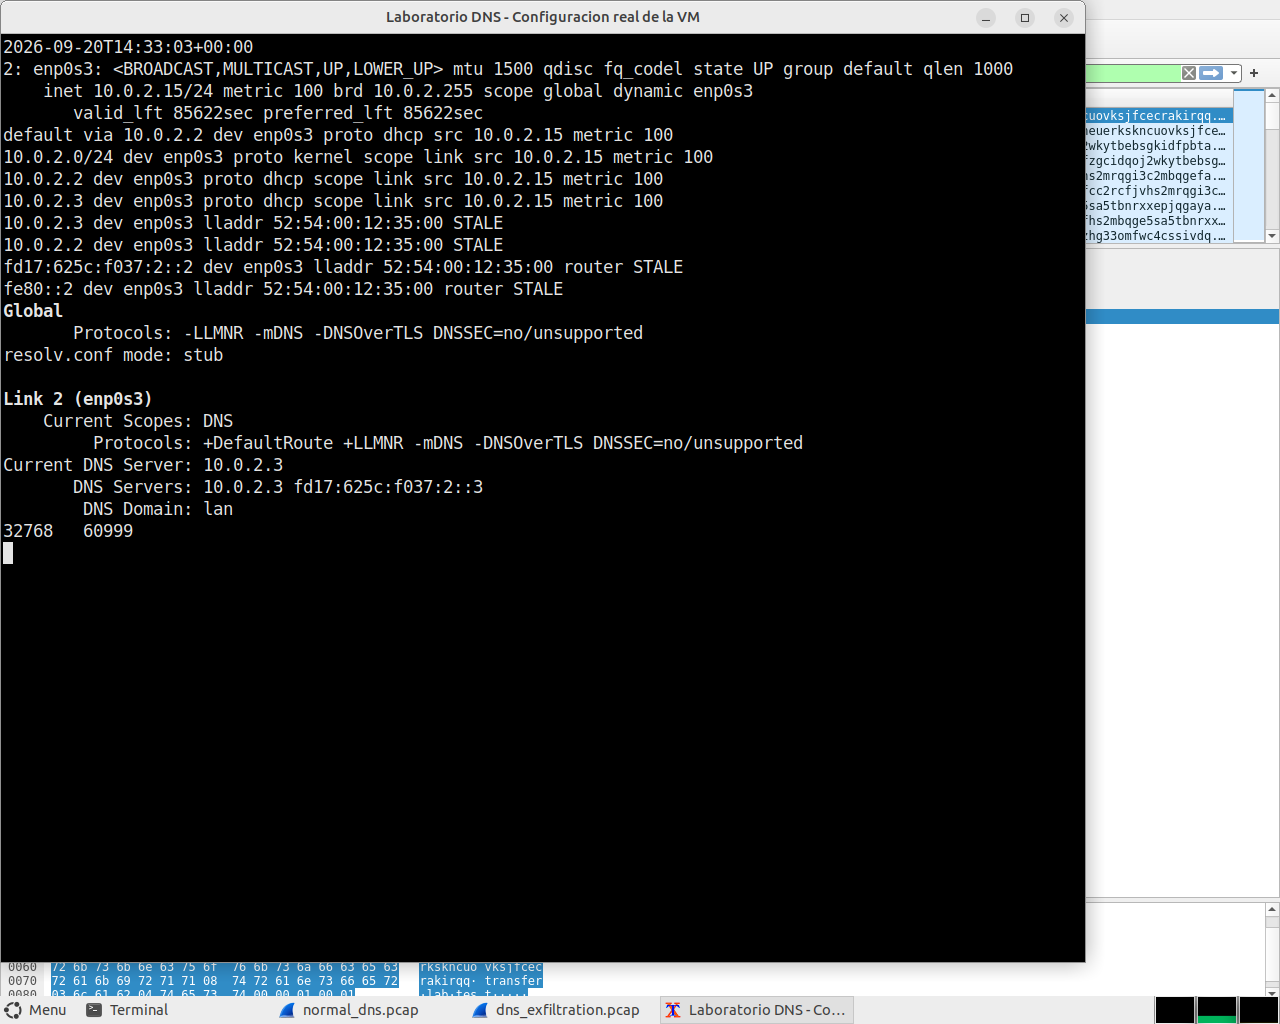
\includegraphics[width=\textwidth]{02_configuracion_red.png}
\caption{Comandos ejecutados en la VM para obtener interfaz, dirección, rutas,
vecinos y servidores DNS.}
\label{fig:configuracion}
\end{figure}
La Figura~\ref{fig:configuracion} muestra que el resolver efectivo es
\nolinkurl{10.0.2.3} y el gateway es \nolinkurl{10.0.2.2}. La tabla de vecinos
asocia ambos con \texttt{52:54:00:12:35:00}, una particularidad observable
del NAT de VirtualBox. No es la MAC física del router doméstico.

Los registros del host usan UTC$-3$ y los de la VM, UTC; por ejemplo,
14:24 UTC equivale a 11:24 en Córdoba. Los PCAP conservan sus timestamps.
La carpeta recibida contenía los dos DOCX, pero no la imagen de la consigna
general mencionada en el texto adjunto. Respondimos las preguntas de los
documentos y las dos preguntas generales transcritas por el usuario.

\section{Laboratorio 17.1.7: explorar tráfico DNS}
\label{sec:lab1}

\subsection{Procedimiento realizado}

Comprobamos que \texttt{systemd-resolved} estaba activo, mientras que
\texttt{dnsmasq} y \texttt{nscd} estaban inactivos. Ejecutamos
\texttt{resolvectl flush-caches}; después, \texttt{resolvectl statistics}
mostró \emph{Current Cache Size: 0}. No fue necesario reiniciar el servicio.
Este vaciado afecta a la caché de la VM, no a las cachés del NAT ni de
resolvers externos.

Iniciamos \texttt{dumpcap}, el componente de captura de Wireshark, sobre
\texttt{enp0s3}, sin filtro de captura y sin modo promiscuo. Abrimos
\texttt{nslookup} en modo interactivo, seleccionamos el DNS del enlace,
consultamos Cisco y finalizamos con \texttt{exit}:

\par\noindent\begin{minipage}{\linewidth}
\begin{lstlisting}
dumpcap -i enp0s3 -p -P -w capturas/normal_dns.pcap
nslookup
> server 10.0.2.3
> www.cisco.com
> exit
\end{lstlisting}
\end{minipage}\par\medskip

Seleccionar explícitamente el servidor evita confundir el intercambio con
el stub de loopback con el tráfico Ethernet que queremos estudiar. Agregamos
consultas A y AAAA de Google, \nolinkurl{example.com} y \nolinkurl{www.iana.org},
y repetimos consultas A de Cisco y Google. El script
\nolinkurl{scripts/normal.py} documenta el orden exacto. Detuvimos la captura
con SIGINT y la abrimos en Wireshark con los filtros \texttt{dns} y
\nolinkurl{udp.port == 53}.

Se guardaron 22 tramas: 10 consultas, 10 respuestas y 2 paquetes ARP.
\texttt{dumpcap} informó cero paquetes descartados. La captura se efectuó
con la herramienta de línea de comandos y el análisis visual con Wireshark
gráfico; las imágenes proceden del framebuffer real de VirtualBox.

\subsection{Consulta y respuesta seleccionadas}

La consulta A de \nolinkurl{www.cisco.com} es la trama 1; su respuesta, la 2.
Coinciden el identificador \texttt{0x669f}, la pregunta y los extremos
invertidos. La diferencia temporal capturada es aproximadamente 157.882 ms.

\begin{table}[H]
\centering\small
\caption{Campos medidos en las tramas 1 y 2 de \nolinkurl{normal_dns.pcap}.}
\begin{tabularx}{\textwidth}{Xll}
\toprule
Campo & Consulta & Respuesta \\
\midrule
Trama & \texttt{1} & \texttt{2} \\
Longitud de trama (bytes) & \texttt{73} & \texttt{201} \\
MAC origen & \texttt{08:00:27:55:44:07} & \texttt{52:54:00:12:35:00} \\
MAC destino & \texttt{52:54:00:12:35:00} & \texttt{08:00:27:55:44:07} \\
IPv4 origen & \texttt{10.0.2.15} & \texttt{10.0.2.3} \\
IPv4 destino & \texttt{10.0.2.3} & \texttt{10.0.2.15} \\
Puerto UDP origen & \texttt{41544} & \texttt{53} \\
Puerto UDP destino & \texttt{53} & \texttt{41544} \\
Longitud IPv4 (bytes) & \texttt{59} & \texttt{187} \\
Longitud UDP (bytes) & \texttt{39} & \texttt{167} \\
Datos DNS (bytes) & \texttt{31} & \texttt{159} \\
Checksum UDP observado & \texttt{0x184a} & \texttt{0x3907} \\
Transaction ID & \texttt{0x669f} & \texttt{0x669f} \\
Flags DNS & \texttt{0x0100} & \texttt{0x8180} \\
\bottomrule
\end{tabularx}

\end{table}

La consulta mide $14+20+8+31=73$ bytes: Ethernet, IPv4, UDP y DNS,
respectivamente. La respuesta mide $14+20+8+159=201$ bytes. Estos tamaños
son los registrados por la captura; no incluyen preámbulo ni intervalo entre
tramas, y no se observó un FCS Ethernet separado en estos paquetes.

\begin{figure}[H]
\centering
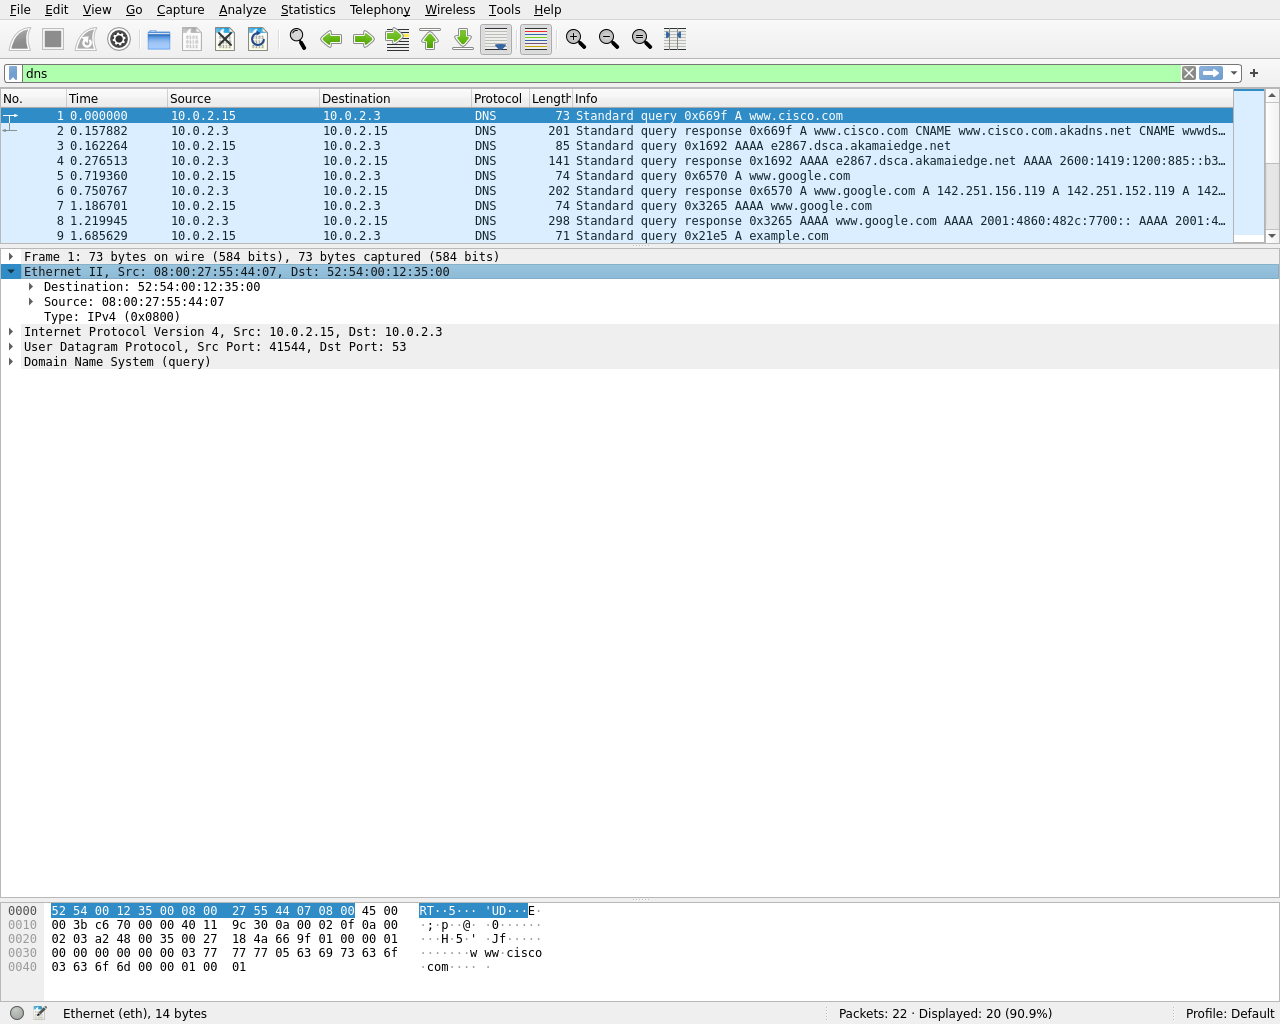
\includegraphics[width=\textwidth]{06_ethernet_query.png}
\caption{Consulta de Cisco con Ethernet II desplegado.}
\label{fig:ethernet}
\end{figure}
En la Figura~\ref{fig:ethernet} la MAC origen coincide con la interfaz
virtual de la estación. La MAC destino pertenece al servicio del NAT
alcanzable en el enlace virtual; el campo Type indica IPv4.

\begin{figure}[H]
\centering
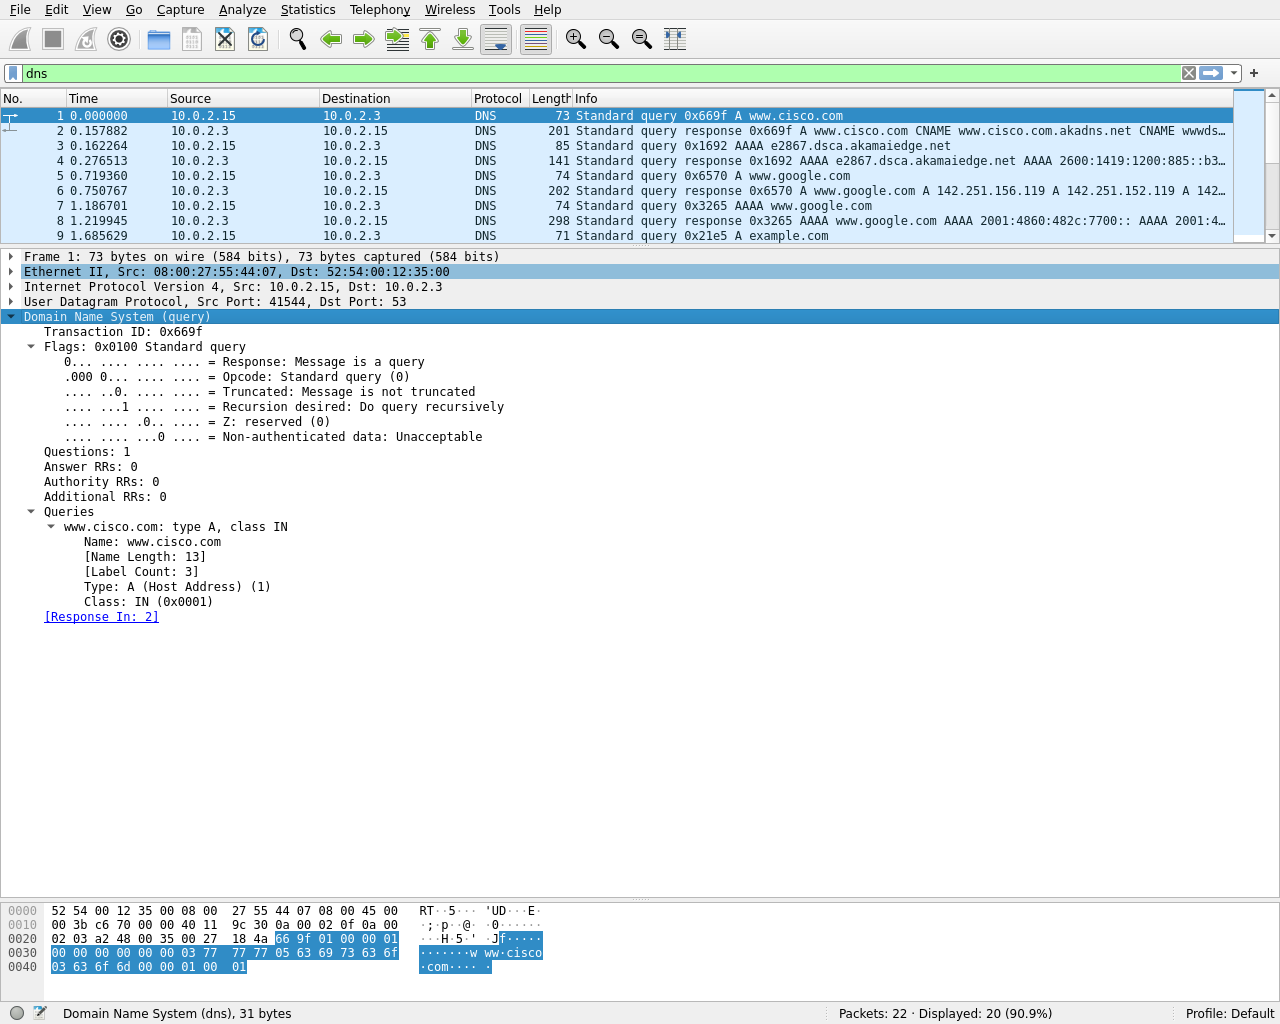
\includegraphics[width=\textwidth]{09_dns_query.png}
\caption{Pregunta DNS de la trama 1, incluidos identificador, flags y tipo A.}
\label{fig:dnsquery}
\end{figure}
En la Figura~\ref{fig:dnsquery} se observa una sola pregunta, sin respuestas
todavía. El flag \texttt{0x0100} representa QR=0 y RD=1: la estación solicita
la resolución recursiva del nombre.

\begin{figure}[H]
\centering
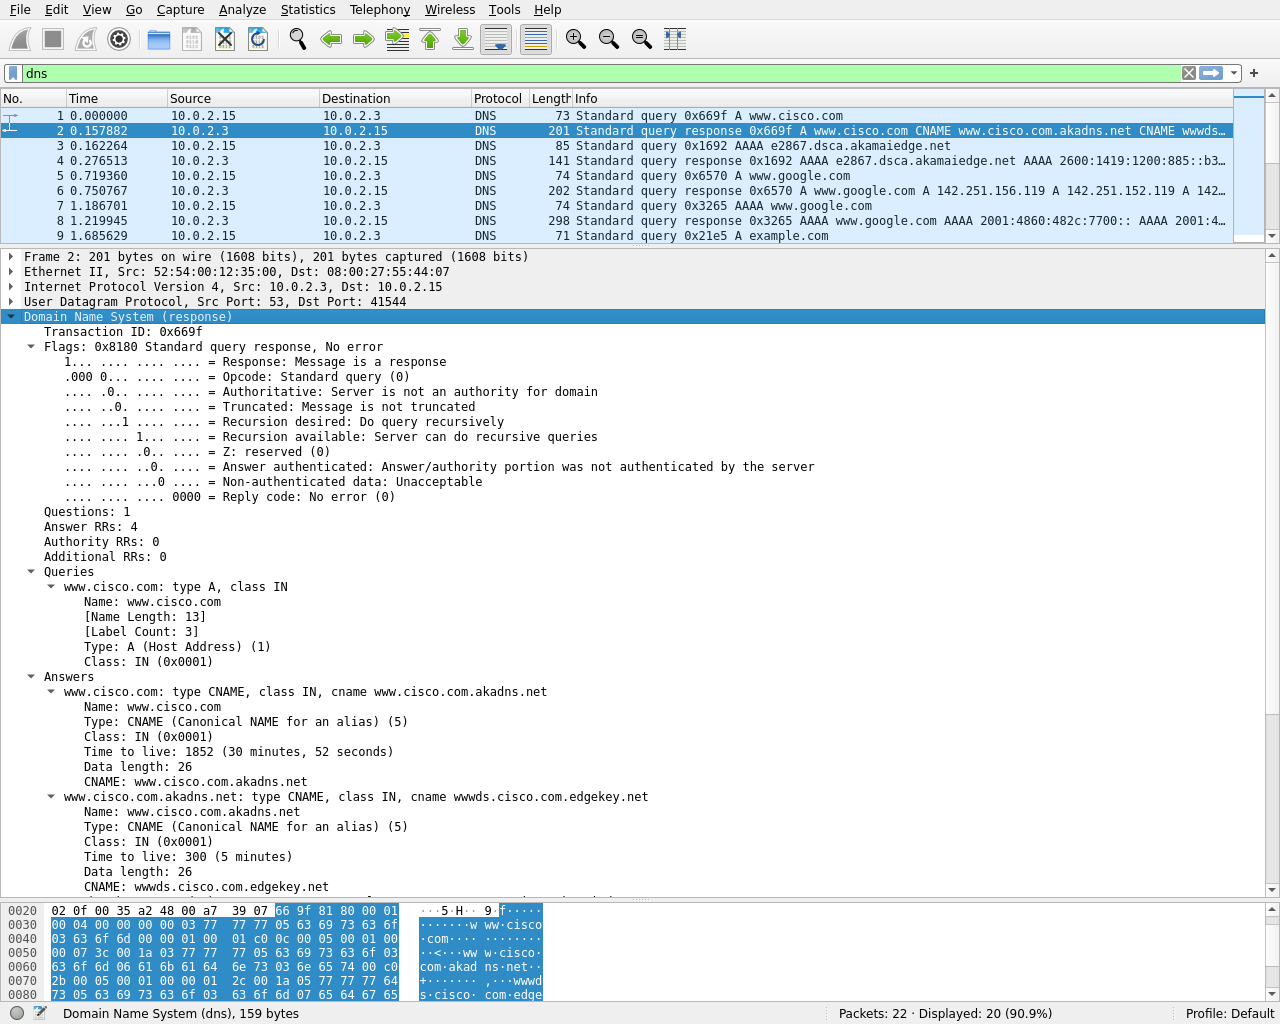
\includegraphics[width=\textwidth]{10_dns_respuesta_cisco.png}
\caption{Respuesta de Cisco con RA=1 y los primeros registros de la cadena CNAME.}
\label{fig:ciscoresponse}
\end{figure}
La Figura~\ref{fig:ciscoresponse} muestra QR=1, RD=1, RA=1 y RCODE=0.
El servidor anuncia recursión y devuelve una respuesta exitosa no autoritativa.
La cadena completa observada en la sección Answers fue:

\begin{enumerate}[noitemsep]
\item \nolinkurl{www.cisco.com} $\rightarrow$ \nolinkurl{www.cisco.com.akadns.net}, CNAME, TTL 1852 s.
\item \nolinkurl{www.cisco.com.akadns.net} $\rightarrow$ \nolinkurl{wwwds.cisco.com.edgekey.net}, CNAME, TTL 300 s.
\item \nolinkurl{wwwds.cisco.com.edgekey.net} $\rightarrow$ \nolinkurl{e2867.dsca.akamaiedge.net}, CNAME, TTL 18169 s.
\item \nolinkurl{e2867.dsca.akamaiedge.net} $\rightarrow$ \nolinkurl{2.20.140.117}, A, TTL 20 s.
\end{enumerate}

\texttt{nslookup} generó además una consulta AAAA del nombre canónico
\nolinkurl{e2867.dsca.akamaiedge.net}, en la trama 3. La respuesta 4 contiene
\texttt{2600:1419:1200:885::b33} y \texttt{2600:1419:1200:884::b33}, ambas
con TTL 20 s. Son direcciones IPv6 dentro de registros DNS; el transporte
de esa consulta siguió siendo IPv4/UDP.

\subsection{Respuestas a todas las preguntas}
\label{sec:respuestas1}
\begin{enumerate}[label=\textbf{\arabic*.},leftmargin=*]
\item \textbf{¿Qué sucedió con las MAC de origen y destino y a qué interfaces
están asociadas?} En la consulta son \texttt{08:00:27:55:44:07} y
\texttt{52:54:00:12:35:00}. La primera es \texttt{enp0s3} de la VM; la
segunda corresponde al extremo virtual que atiende el DNS del NAT. En la
respuesta se invierten. No son las MAC de los servidores web de Cisco.

\item \textbf{¿Cuáles son las IP de origen y destino y a qué interfaces
están asociadas?} La consulta sale de \nolinkurl{10.0.2.15}, asignada a
\texttt{enp0s3}, hacia \nolinkurl{10.0.2.3}, el proxy/resolver DNS anunciado
por la red virtual. No se dirige a la IP obtenida para la web.

\item \textbf{¿Cuáles son los puertos de origen y destino? ¿Cuál es el
predeterminado de DNS?} En la trama 1 son 41544 y 53. El primero es el
puerto efímero del cliente; el segundo es el puerto convencional de DNS.

\item \textbf{¿Qué resulta de comparar MAC e IP de Wireshark con las del
terminal?} La MAC y la IP origen coinciden exactamente con
\texttt{ip addr show enp0s3}. La IP destino coincide con
\texttt{resolvectl status}, y su MAC con \texttt{ip neigh}. Esto confirma
que capturamos la interfaz y el intercambio esperados.

\item \textbf{¿Cuáles son MAC, IP y puertos de la respuesta? ¿Qué cambia?}
La trama 2 sale de MAC \texttt{52:54:00:12:35:00}, IP \nolinkurl{10.0.2.3}
y puerto 53, hacia MAC \texttt{08:00:27:55:44:07}, IP \nolinkurl{10.0.2.15}
y puerto 41544. Se invierten los extremos; el ID y la pregunta se conservan,
QR pasa a 1 y aparecen cuatro registros de respuesta.

\item \textbf{¿El servidor DNS puede realizar consultas recursivas?}
Sí: RA=1 anuncia que el servicio ofrece recursión. El PCAP del cliente
no permite determinar si esta respuesta requirió recorrer la jerarquía,
si fue reenviada a otro resolver o si se obtuvo de una caché.

\item \textbf{¿Qué similitudes y diferencias existen con nslookup?}
La salida coincide en la cadena de alias y en las direcciones A y AAAA.
\texttt{nslookup} resume la resolución, mientras Wireshark separa las
transacciones, sus flags, TTL, puertos y longitudes. Los AAAA que aparecen
en la salida del comando proceden de la respuesta 4, no de la respuesta A
de la trama 2.

\item \textbf{Sin el filtro, ¿qué más podemos averiguar sobre la red?}
En esta captura aparecen las tramas ARP 21 y 22, que permiten observar la
resolución de un vecino IPv4 a una MAC. En otras capturas podrían verse
DHCP, descubrimiento IPv6, conexiones TCP y destinos de aplicaciones, según
el punto de observación. No afirmamos que esos otros protocolos estén en
la muestra normal obtenida.

\item \textbf{¿Cómo podría un atacante utilizar Wireshark para comprometer
la seguridad?} Con acceso a un punto de captura podría reconocer servicios,
resolver nombres de interés y examinar datos transmitidos sin cifrar. En
una red con switches no ve automáticamente todo el tráfico de los demás
equipos, y TLS no se descifra por el solo hecho de capturarlo. Deben
protegerse los endpoints y los permisos de captura y evitar protocolos
que transmitan información sensible en claro.
\end{enumerate}

\section{Laboratorio 10.2.7: examinar una captura DNS sobre UDP}
\label{sec:lab2}

\subsection{Procedimiento y tablas solicitadas}

La configuración de la Parte 1 está completa en la
Tabla~\ref{tab:configuracion}. No ejecutamos el script DHCP de la antigua
imagen porque la estación ya tenía dirección y ruta. Para la Parte 2
utilizamos \texttt{dig} como alternativa al navegador, autorizada por la
consigna general. No se presenta una apertura de Google en Firefox como
actividad realizada. El comando efectivamente ejecutado fue:

\par\noindent\begin{minipage}{\linewidth}
\begin{lstlisting}
dig @10.0.2.3 www.google.com A +noedns +time=3 +tries=1
\end{lstlisting}
\end{minipage}\par\medskip

La consulta y su respuesta son las tramas 5 y 6 del mismo PCAP. Reutilizar
la captura conserva la numeración original y permite comparar ambos
laboratorios. No se copiaron las tramas 429/488 ni los puertos del ejemplo
del documento de Cisco.

\begin{table}[H]
\centering\small
\caption{Identificación de dispositivos; segunda tabla del DOCX 10.2.7.}
\begin{tabularx}{\textwidth}{Xll}
\toprule
Dispositivo & Dirección IP & Dirección MAC \\
\midrule
Estación cliente & \nolinkurl{10.0.2.15} & \texttt{08:00:27:55:44:07} \\
Destino DNS del NAT & \nolinkurl{10.0.2.3} & \texttt{52:54:00:12:35:00} \\
Gateway, como referencia & \nolinkurl{10.0.2.2} & \texttt{52:54:00:12:35:00} \\
\bottomrule
\end{tabularx}
\end{table}

El DNS de nuestra VM está en el enlace virtual local. La explicación del
DOCX según la cual la MAC destino siempre es la del gateway corresponde a
su ejemplo con un DNS remoto. En nuestro caso el NAT utiliza la misma MAC
para sus servicios DNS y gateway, pero las IP siguen siendo diferentes.

\begin{table}[H]
\centering\small
\caption{Tercera tabla del DOCX, ampliada con la respuesta y los campos de UDP/DNS.}
\begin{tabularx}{\textwidth}{Xll}
\toprule
Campo & Consulta & Respuesta \\
\midrule
Trama & \texttt{5} & \texttt{6} \\
Longitud de trama (bytes) & \texttt{74} & \texttt{202} \\
MAC origen & \texttt{08:00:27:55:44:07} & \texttt{52:54:00:12:35:00} \\
MAC destino & \texttt{52:54:00:12:35:00} & \texttt{08:00:27:55:44:07} \\
IPv4 origen & \texttt{10.0.2.15} & \texttt{10.0.2.3} \\
IPv4 destino & \texttt{10.0.2.3} & \texttt{10.0.2.15} \\
Puerto UDP origen & \texttt{48201} & \texttt{53} \\
Puerto UDP destino & \texttt{53} & \texttt{48201} \\
Longitud IPv4 (bytes) & \texttt{60} & \texttt{188} \\
Longitud UDP (bytes) & \texttt{40} & \texttt{168} \\
Datos DNS (bytes) & \texttt{32} & \texttt{160} \\
Checksum UDP observado & \texttt{0x184b} & \texttt{0x6986} \\
Transaction ID & \texttt{0x6570} & \texttt{0x6570} \\
Flags DNS & \texttt{0x0120} & \texttt{0x8180} \\
\bottomrule
\end{tabularx}

\label{tab:google}
\end{table}

Los tres objetos de tabla editables del DOCX quedan así completos: configuración,
identificación de dispositivos y campos de la consulta. La columna de respuesta
de la Tabla~\ref{tab:google} se agrega para comprobar la inversión de los extremos.

\begin{figure}[H]
\centering
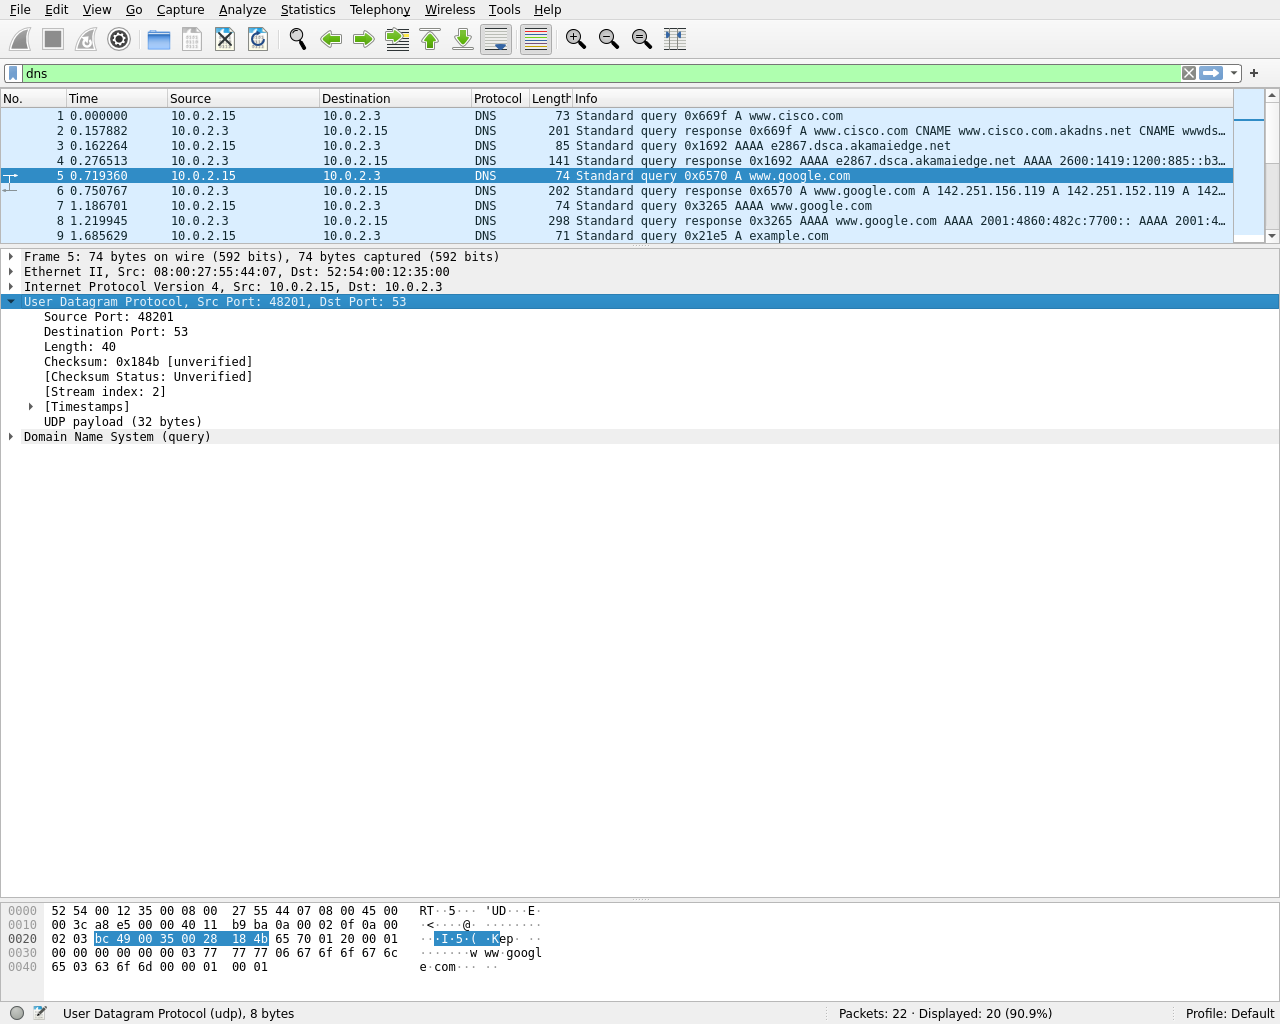
\includegraphics[width=\textwidth]{12_google_consulta_udp.png}
\caption{Trama 5: consulta A de Google con los cuatro campos de UDP desplegados.}
\label{fig:googleudp}
\end{figure}
La Figura~\ref{fig:googleudp} permite separar los 40 bytes de UDP en 8 bytes
de cabecera y 32 de datos DNS. La trama completa mide 74 bytes. La respuesta
mide 202 bytes porque incorpora ocho registros A, además de repetir la pregunta.

Los flags de la consulta son \texttt{0x0120}: RD=1 y AD=1. En una consulta,
AD señala que el cliente entiende ese bit; no significa que la pregunta esté
autenticada. La respuesta tiene \texttt{0x8180}, con AD=0, de modo que no
aporta evidencia de validación DNSSEC~\cite{rfc6840}. El RTT medido entre las
tramas 5 y 6 es 31.407 ms; la salida de \texttt{dig} informó 32 ms.

En la respuesta 6 se observaron estos ocho registros A, todos con TTL 119 s:
\nolinkurl{142.251.156.119}, \nolinkurl{142.251.152.119},
\nolinkurl{142.251.154.119}, \nolinkurl{142.251.151.119},
\nolinkurl{142.251.155.119}, \nolinkurl{142.251.150.119},
\nolinkurl{142.251.157.119} y \nolinkurl{142.251.153.119}.
La respuesta AAAA posterior, trama 8, contiene ocho direcciones IPv6;
se conservan completas en \nolinkurl{normal_dns_paquetes.json}. La presencia
de varias direcciones es un resultado observado, no una garantía de que
se obtengan las mismas en una ejecución futura.

Los checksums mostrados en las tablas son los bytes capturados. Wireshark
los presenta como no verificados cuando la validación está deshabilitada.
La descarga del cálculo de checksums hacia la interfaz puede dejar valores
parciales en una captura de salida; un aparente checksum incorrecto en ese
punto no basta para concluir que hubo corrupción~\cite{checksums}.

\subsection{Respuestas a todas las preguntas}
\label{sec:respuestas2}
\begin{enumerate}[label=\textbf{\arabic*.},leftmargin=*]
\item \textbf{¿La MAC origen es la misma que la registrada para la VM?}
Sí: \texttt{08:00:27:55:44:07} tanto en la configuración como en la trama 5.

\item \textbf{¿Se pueden identificar las IP y MAC de origen y destino?}
Sí. Origen: \nolinkurl{10.0.2.15} y \texttt{08:00:27:55:44:07}.
Destino: \nolinkurl{10.0.2.3} y \texttt{52:54:00:12:35:00}. La tabla de
dispositivos documenta la diferencia entre DNS y gateway.

\item \textbf{¿La IP origen es la IP local registrada en la Parte 1?}
Sí, \nolinkurl{10.0.2.15}. Es la IP de la VM y no la del host físico.

\item \textbf{¿La IP destino coincide con el gateway predeterminado?}
No. El destino es \nolinkurl{10.0.2.3}, mientras que el gateway es
\nolinkurl{10.0.2.2}. La coincidencia de sus MAC en el NAT no los convierte
en la misma dirección IP.

\item \textbf{En la respuesta Ethernet II, ¿a qué dispositivos corresponden
las MAC?} Origen \texttt{52:54:00:12:35:00}: servicio DNS del NAT;
destino \texttt{08:00:27:55:44:07}: adaptador \texttt{enp0s3} de la VM.

\item \textbf{¿Cuál es la IP destino de la respuesta?}
\nolinkurl{10.0.2.15}, la estación que generó la consulta.

\item \textbf{¿Cuál es la IP origen de la respuesta?}
\nolinkurl{10.0.2.3}, el servidor DNS consultado.

\item \textbf{¿Qué ocurrió con los roles de origen y destino de la VM y
del gateway?} Se invirtieron los extremos de la conversación y de la trama.
En nuestra topología el interlocutor IP es el DNS \nolinkurl{10.0.2.3}; no
debe sustituirse por el gateway \nolinkurl{10.0.2.2}. Los puertos cambian de
$48201\rightarrow53$ a $53\rightarrow48201$.

\item \textbf{Reflexión: ¿qué ventajas tiene UDP frente a TCP para DNS?}
Una consulta breve puede resolverse con una solicitud y una respuesta, sin
establecer antes una conexión y con una cabecera de transporte pequeña.
Esto reduce intercambios y estado mantenido. UDP no garantiza entrega ni
orden: los reintentos y temporizadores quedan a cargo de la aplicación.
TCP sigue siendo necesario en DNS y puede reutilizar conexiones, por lo que
la comparación no debe reducirse a ``TCP siempre es lento''.
\end{enumerate}

\section{Exfiltración y tunneling mediante DNS}

La exfiltración mediante DNS consiste en trasladar información dentro de
mensajes DNS hacia un receptor que puede recuperarla. El artículo de Helge
Klein describe dos recorridos: enviar directamente al servidor del receptor
o utilizar la cadena de resolución habitual para llegar a un dominio bajo
su control. En ambos, los subdominios transportan fragmentos codificados.
En el segundo recorrido, el servidor autoritativo del dominio recibe las
preguntas reenviadas y puede extraer los datos. La variante directa puede
bloquearse restringiendo los resolvers permitidos; la indirecta exige también
controlar el contenido que procesa el resolver autorizado~\cite{klein}.

La razón del abuso no es una vulnerabilidad de UDP: una política que permita
resolver nombres arbitrarios ya habilita un intercambio de información. Un
túnel DNS utiliza ese intercambio como transporte para otra comunicación,
incluso bidireccional. Exfiltrar un archivo es un uso posible de ese canal;
no toda exfiltración implementa un túnel general. MITRE ATT\&CK contempla DNS
entre los protocolos que pueden transportar datos extraídos~\cite{mitre}.

El artículo utiliza DNSteal y una variante con codificación hexadecimal.
Adaptamos el concepto a una implementación educativa en Python 3 ya disponible,
con Base32 y un único archivo sintético fijo. No ejecutamos DNSteal, no
instalamos Python 2 y no modificamos el resolver del sistema para liberar su
puerto~\cite{klein}.

\subsection{Topología realmente utilizada}

Dentro de la VM creamos dos espacios de nombres de red Linux
(\emph{network namespaces}), con interfaces, rutas y sockets separados,
unidos mediante un par \texttt{veth}. Son dos entornos de red dentro del
mismo kernel, no dos máquinas virtuales independientes. Los nombres y
direcciones siguientes se asignaron efectivamente y quedaron registrados
por los comandos y por el PCAP:

\begin{center}
\fbox{\begin{minipage}{0.91\textwidth}
\centering
VM Cisco: red experimental separada de \texttt{enp0s3}\\[6pt]
\texttt{dns-client-20260920}\quad $\longleftrightarrow$\quad
\texttt{dns-server-20260920}\\
\nolinkurl{dns-cli: 10.203.0.1/30}\qquad
\nolinkurl{dns-rx: 10.203.0.2/30}\\[6pt]
Par Ethernet virtual; sin gateway ni ruta predeterminada en ambos namespaces.
\end{minipage}}
\end{center}

El emisor contacta directamente con \nolinkurl{10.203.0.2:53}. El receptor sólo
escucha en esa IP y verifica la IP del emisor. No hay interfaz compartida
con la LAN ni una ruta hacia el NAT de la VM. El sufijo elegido fue
\nolinkurl{transfer.lab.test}; \nolinkurl{.test} está reservado para pruebas
según RFC 2606~\cite{rfc2606}. La reserva del nombre evita colisiones, pero
el aislamiento lo proporcionan las interfaces y rutas, no el sufijo por sí solo.

\subsection{Archivo, transferencia y reconstrucción}

El script \nolinkurl{dns_demo.py} creó un archivo de 1072 bytes que comienza
con el siguiente contenido y continúa con 16 registros numerados, todos ficticios:

\par\noindent\begin{minipage}{\linewidth}
\begin{lstlisting}
LABORATORIO DE CIBERSEGURIDAD
Datos ficticios para prueba de exfiltracion DNS.
ID-DEMO-2026-001
REGISTRO-FICTICIO-001; valor=0007; sin informacion personal.
\end{lstlisting}
\end{minipage}\par\medskip

El programa sólo lee el contenido sintético definido en su propio código;
no recibe una ruta de archivo arbitraria. Dividió los datos en 33 bloques
de 32 bytes y uno final de 16 bytes. Cada bloque se codificó en Base32 sin
relleno y se incorporó a una pregunta A con esta estructura:

\par\noindent\begin{minipage}{\linewidth}
\begin{lstlisting}
s0000.n0034.<bloque_base32>.transfer.lab.test
\end{lstlisting}
\end{minipage}\par\medskip

La primera etiqueta indica la secuencia y la segunda el total de bloques.
La tercera contiene los datos. Un bloque completo ocupa 52 caracteres
Base32, dentro del máximo de una etiqueta; el nombre completo mide 82
caracteres sin el punto final. Base32 permite utilizar letras y dígitos
del 2 al 7, y se normalizó a minúsculas. No es cifrado: cualquiera que
capture las preguntas y conozca el formato puede decodificar su contenido.
Hexadecimal también sería posible, con más expansión; Base64 convencional
contiene caracteres y diferencias de mayúsculas que exigen más cuidado en
un nombre DNS.

El receptor obtiene el índice, decodifica el bloque, lo almacena y devuelve
una respuesta A inocua con \nolinkurl{10.203.0.2}, TTL 0, AA=1 y RA=0. El emisor
valida el identificador de la respuesta y espera 0.2 s antes del bloque
siguiente. El ID DNS se genera para cada consulta; no sustituye al índice
del archivo. No implementamos una herramienta general de túneles, reintentos
ante pérdida ni transferencia de documentos del usuario.

La recepción une los bloques por su índice. Además, \nolinkurl{analizar.py}
reconstruye el archivo exclusivamente desde las preguntas del PCAP. Se
compararon byte a byte el original, el archivo del receptor y el recuperado
de la captura. Los tres tienen 1072 bytes y este SHA-256:

\begin{center}\small\ttfamily
41e631070a6cf404f57bf882d7e1161af41\\
f816e5660468d7aac6630dd22a731
\end{center}

El salto de línea anterior sólo facilita la lectura del hash de 64 dígitos.
La coincidencia permite verificar la integridad de estos archivos; no es
una autenticación de un remitente ni una protección del canal.

\subsection{Captura y análisis del intercambio}

El PCAP definitivo contiene 83 tramas, de las cuales 34 son consultas DNS,
34 respuestas y 15 tráfico auxiliar de Ethernet/IPv6. Todas las preguntas
de la transferencia utilizan A y UDP. Se registraron cero descartes.
La primera pareja DNS es la de las tramas 6 y 7:

\begin{table}[H]
\centering\small
\caption{Primera consulta y respuesta de \nolinkurl{dns_exfiltration.pcap}.}
\begin{tabularx}{\textwidth}{Xll}
\toprule
Campo & Consulta & Respuesta \\
\midrule
Trama & \texttt{6} & \texttt{7} \\
Longitud de trama (bytes) & \texttt{142} & \texttt{158} \\
MAC origen & \texttt{7e:9e:18:cd:b2:18} & \texttt{02:af:b9:5b:09:ac} \\
MAC destino & \texttt{02:af:b9:5b:09:ac} & \texttt{7e:9e:18:cd:b2:18} \\
IPv4 origen & \texttt{10.203.0.1} & \texttt{10.203.0.2} \\
IPv4 destino & \texttt{10.203.0.2} & \texttt{10.203.0.1} \\
Puerto UDP origen & \texttt{37400} & \texttt{53} \\
Puerto UDP destino & \texttt{53} & \texttt{37400} \\
Longitud IPv4 (bytes) & \texttt{128} & \texttt{144} \\
Longitud UDP (bytes) & \texttt{108} & \texttt{124} \\
Datos DNS (bytes) & \texttt{100} & \texttt{116} \\
Checksum UDP observado & \texttt{0x1616} & \texttt{0x1626} \\
Transaction ID & \texttt{0x24ee} & \texttt{0x24ee} \\
Flags DNS & \texttt{0x0000} & \texttt{0x8400} \\
\bottomrule
\end{tabularx}

\end{table}

Las MAC de las interfaces experimentales se generaron al crear el par
\texttt{veth}: cliente \texttt{7e:9e:18:cd:b2:18} y receptor
\texttt{02:af:b9:5b:09:ac}. No se utilizaron como ejemplos escritos antes
de ejecutar la red. El puerto efímero observado fue 37400 y se mantuvo
durante la transferencia porque el emisor reutilizó el socket.

\begin{figure}[H]
\centering
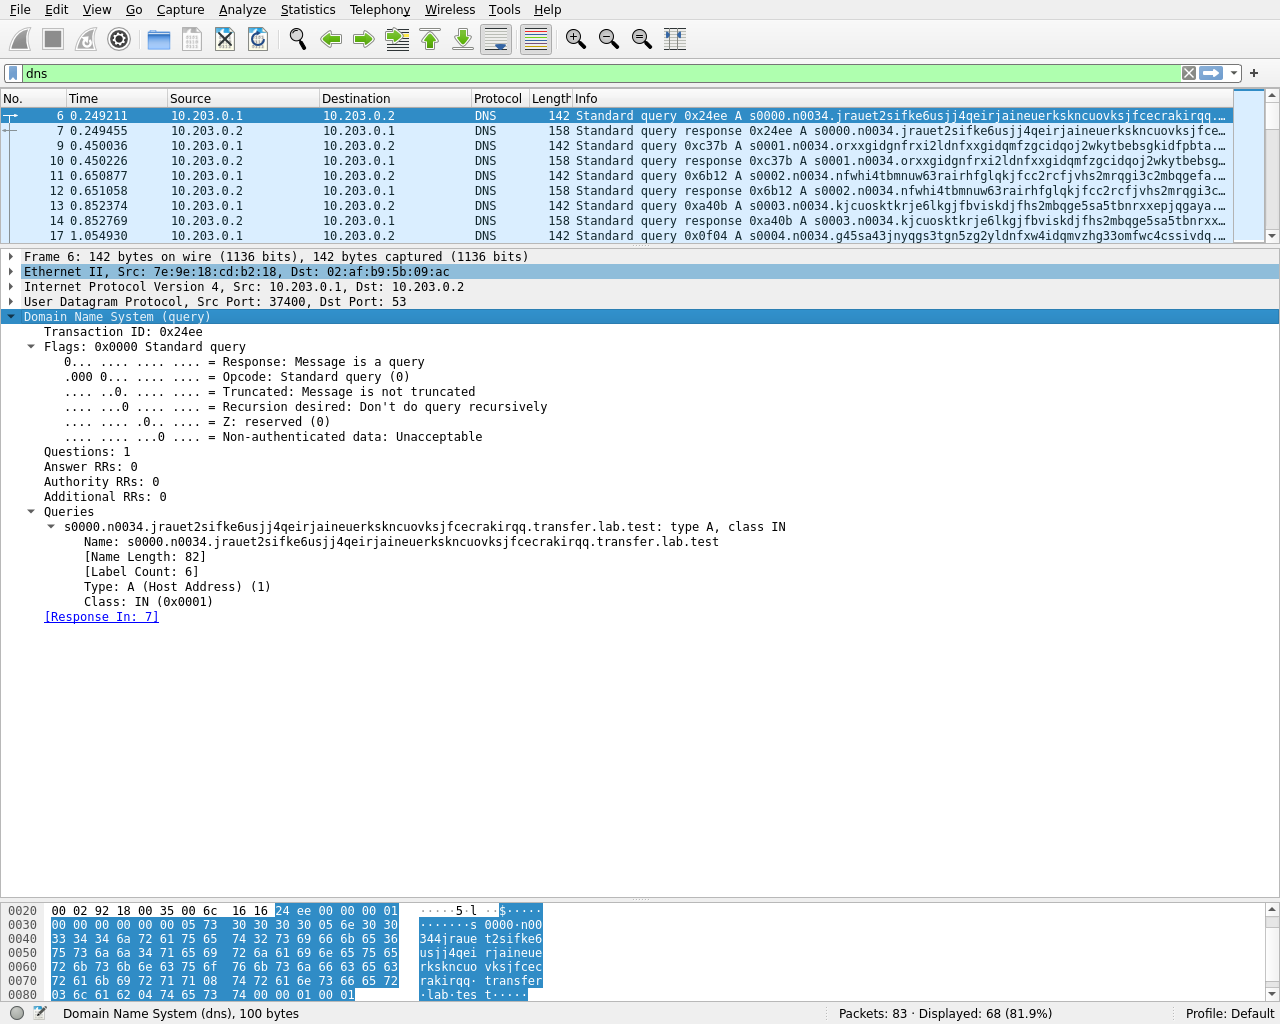
\includegraphics[width=\textwidth]{15_exfiltracion_consulta.png}
\caption{Pregunta real de exfiltración, trama 6, con el bloque Base32 en el nombre.}
\label{fig:exfil}
\end{figure}
En la Figura~\ref{fig:exfil} se observan seis etiquetas y un nombre de 82
caracteres. El mensaje tiene forma de consulta A, pero su nombre transporta
parte del archivo. RD=0 porque el cliente se comunica directamente con el
receptor del laboratorio; no solicita recursión.

\begin{figure}[H]
\centering
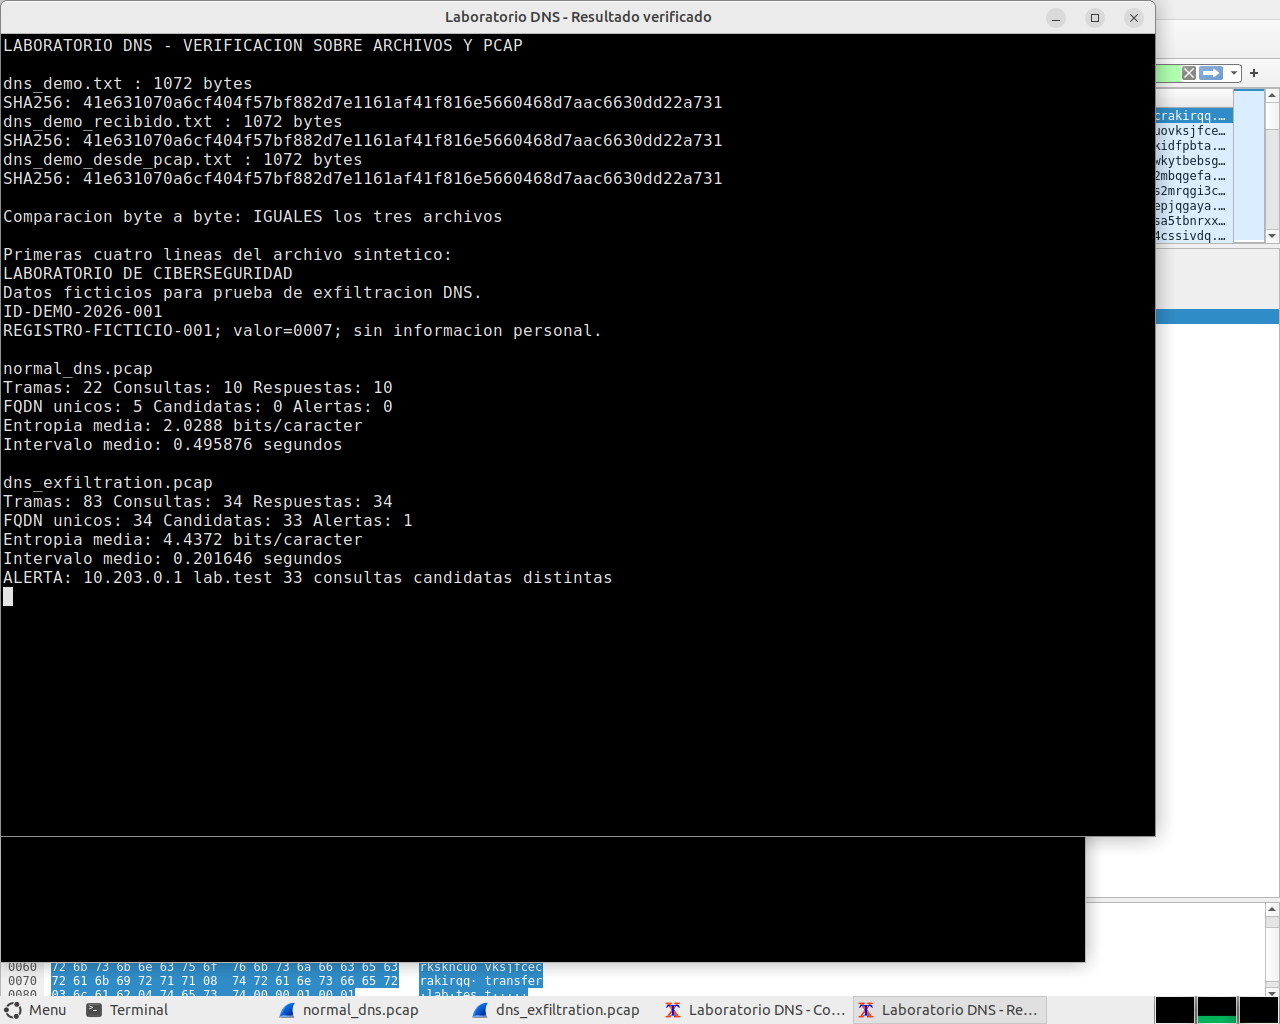
\includegraphics[width=\textwidth]{16_verificacion.png}
\caption{Verificación en terminal de los archivos y del resultado de detección.}
\label{fig:verificacion}
\end{figure}
La Figura~\ref{fig:verificacion} muestra la comparación del original y la
recepción, junto con las métricas obtenidas del PCAP. La reconstrucción desde
las preguntas demuestra que los datos ya viajaban en la solicitud: una
respuesta DNS de error tampoco habría retirado lo enviado.

\subsection{Incidencia registrada y límites de la prueba}

El primer intento transfirió el archivo, pero \texttt{dumpcap} falló al abrir
el archivo de salida con \emph{Permission denied}. No consideramos ese
intento una demostración respaldada por PCAP. Conservamos su registro en
\nolinkurl{resultados/vm/intento_01/}. En el segundo intento abrimos el archivo
desde el proceso coordinador y utilizamos \texttt{dumpcap -w -}, redirigiendo
su salida binaria a ese archivo. También incorporamos una comprobación de
que el capturador siguiera activo antes de enviar los datos y una verificación
de salida y tamaño al finalizar. Esta ejecución produjo el PCAP analizado.
No se atribuyó el fallo a una causa específica de permisos sin verificarla.

Al terminar eliminamos los dos namespaces creados; \texttt{ip netns list}
quedó vacío. La prueba no envió datos sintéticos a Internet, no publicó un
servidor ni atacó infraestructura de terceros. Las consultas a nombres
públicos pertenecen únicamente a la resolución normal de los laboratorios.
No se ensayó la variante con delegación autoritativa pública, ni un túnel
bidireccional general, ni un IDS desplegado en una red productiva.

\section{Comparación y detección de la exfiltración}
\label{sec:deteccion}

\subsection{Medidas obtenidas de los PCAP}

\begin{table}[H]
\centering\small
\caption{Comparación de las dos muestras capturadas.}
\begin{tabularx}{\textwidth}{Xrr}
\toprule
Medida & Normal & Demostración \\
\midrule
Tramas totales & 22 & 83 \\
Consultas DNS & 10 & 34 \\
Respuestas DNS & 10 & 34 \\
FQDN distintos & 5 & 34 \\
Etiqueta más larga (caracteres) & 10 & 52 \\
Bytes de consultas (Ethernet incluido) & 739 & 4802 \\
Bytes DNS, ambos sentidos (Ethernet incluido) & 2568 & 10148 \\
Respuestas NXDOMAIN & 0 & 0 \\
Consultas candidatas de la heurística & 0 & 33 \\
Longitud FQDN (caracteres) & 11--25 & 56--82 \\
Longitud de consulta (bytes de trama) & 71--85 & 116--142 \\
Entropía media de etiqueta (bits/carácter) & 2.0288 & 4.4372 \\
Intervalo medio entre consultas (s) & 0.4959 & 0.2016 \\
Desvío poblacional del intervalo (s) & 0.1263 & 0.0009 \\
Tasa entre primera y última consulta (s$^{-1}$) & 2.0166 & 4.9592 \\
\bottomrule
\end{tabularx}

\label{tab:comparacion}
\end{table}

La longitud del FQDN se mide en su representación textual, sin punto final;
la entropía se calcula sobre la etiqueta más larga de cada pregunta,
normalizada a minúsculas. Para una etiqueta con frecuencias relativas $p_i$:
\[
H=-\sum_i p_i\log_2 p_i.
\]
Se usa el estimador empírico, sin corrección por tamaño de muestra. La
entropía no demuestra cifrado ni malicia: es una característica para combinar
con otras. El máximo teórico de un alfabeto Base32 uniforme es 5 bits por
carácter, pero nuestros bloques son texto estructurado y no tienen por qué
alcanzarlo.

La muestra normal contiene cinco nombres distintos: Cisco, el nombre canónico
consultado por \texttt{nslookup}, Google, \nolinkurl{example.com} e IANA. La
demostración contiene 34 nombres únicos bajo un mismo sufijo. Su intervalo
medio es 0.2016 s y su desvío poblacional 0.00094 s, coherente con la pausa
programada. La tasa se calculó como $(N-1)/(t_N-t_1)$; no se dividió por
una duración arbitraria de captura.

Los tamaños de las consultas aumentaron de 71--85 a 116--142 bytes.
No se observaron paquetes DNS excepcionalmente grandes respecto de los
límites del protocolo: lo que cambia es su relación con nuestra muestra
normal. Tampoco apareció NXDOMAIN en ninguna muestra. La demo devolvió
respuestas exitosas, de modo que una regla basada únicamente en errores no
la habría detectado.

Las dos muestras son pequeñas y fueron generadas mediante scripts. La
frecuencia de la muestra normal tampoco representa el comportamiento de
una organización. Estas medidas comparan nuestras ejecuciones; no establecen
umbrales universales ni tasas de falsos positivos para producción.

\begin{samepage}
\subsection{Detección ejecutada}

\nolinkurl{scripts/analizar.py} lee los PCAP originales y marca como candidata
una consulta cuya etiqueta más larga cumpla simultáneamente:
\begin{itemize}[noitemsep]
\item longitud de al menos 40 caracteres;
\item entropía de al menos 3.5 bits por carácter;
\item caracteres compatibles con \texttt{[a-z2-7]+}.
\end{itemize}
\end{samepage}
Agrupa por IP origen y por las dos últimas etiquetas del nombre, y genera
una alerta si encuentra al menos cinco preguntas candidatas distintas en
la captura. Para estos nombres el agrupamiento sirve; una herramienta
general debería utilizar una lista de sufijos públicos y ventanas temporales
explícitas, además de separar correctamente clientes detrás de NAT.

El resultado fue una alerta para \nolinkurl{10.203.0.1}, sufijo
\nolinkurl{lab.test}, con 33 consultas candidatas únicas. No generó alertas
en \nolinkurl{normal_dns.pcap}. La trama 82, correspondiente al último bloque,
contiene una etiqueta de 26 caracteres y queda fuera del umbral. Por tanto,
la cobertura sobre las preguntas conocidas de esta transferencia fue
$33/34\approx97.1\%$; no debe interpretarse como una tasa general de detección.

El detector procesa la captura completa: en un sistema en línea sólo podría
disparar tras acumular suficiente evidencia y parte de los datos ya podría
haber salido. Las listas completas de tramas y métricas quedan en
\nolinkurl{resultados/analisis.json} y los CSV. Para repetir el análisis:
\par\noindent\begin{minipage}{\linewidth}
\begin{lstlisting}
python3 scripts/analizar.py
python3 scripts/contrastar_rawshark.py
\end{lstlisting}
\end{minipage}\par\medskip

También ejecutamos, mediante \texttt{rawshark}, este filtro de visualización
de Wireshark sobre la captura de la demostración:
\par\noindent\begin{minipage}{\linewidth}
\begin{lstlisting}
dns.flags.response == 0 && len(dns.qry.name) > 60
\end{lstlisting}
\end{minipage}\par\medskip
Selecciona las 33 preguntas completas de 82 caracteres y excluye el último
nombre de 56. El resultado se conserva en \nolinkurl{filtro_longitud.txt}.
\texttt{rawshark} imprime un indicador final de coincidencia por trama;
contar todas sus líneas como coincidencias daría un resultado incorrecto.
Esta selección por longitud es un apoyo visual, no una confirmación de ataque.

\subsection{Cómo aplicar la detección en una red real}

Se necesitan varias señales y contexto. Conviene medir por host y dominio
la longitud de nombres y etiquetas, la diversidad de subdominios, la
proporción de consultas únicas, el volumen y los intervalos. Secuencias
con alta diversidad y destino concentrado merecen investigación. También
interesan cambios respecto del historial del equipo, dominios poco frecuentes
y alfabetos compatibles con codificaciones. Una CDN o un producto de
telemetría puede producir nombres largos legítimos, por lo que no alcanza
una sola de esas señales.

NXDOMAIN elevado puede acompañar una transferencia sin respuestas válidas
o un algoritmo de generación de dominios, pero también errores de
configuración. TXT o tipos poco habituales pueden ser relevantes, aunque
nuestra transferencia utilizó exclusivamente A. La periodicidad y el volumen
son señales útiles; una extracción lenta puede parecer poco voluminosa y
exige observar ventanas más largas.

Zeek puede registrar en \nolinkurl{dns.log} cliente, servidor, pregunta, tipo,
resultado, flags y respuestas. Esos eventos pueden agregarse en un SIEM
para relacionar una secuencia DNS con otros eventos del endpoint~\cite{zeek}.
Suricata dispone de campos y buffers específicos de DNS, incluido
\nolinkurl{dns.query}, que permiten implementar reglas de contenido y combinar
alertas con umbrales de frecuencia~\cite{suricata}. Aquí no ejecutamos Zeek
ni Suricata: la detección práctica fue Python más el filtro de Wireshark.

Los logs del resolver y un DNS firewall aportan visibilidad cuando no se
dispone de un sensor en cada segmento. La correlación con EDR ayuda a
identificar el proceso que generó las consultas; NDR analiza su comportamiento
en la red. Un modelo estadístico o de aprendizaje automático podría combinar
características, pero necesitaría datos representativos, validación fuera
de muestra y revisión de falsos positivos. No se entrenó un modelo con estas
44 consultas porque no constituyen un conjunto representativo.
\section{Medidas para evitar o mitigar la exfiltración}

Estas medidas se proponen para una red administrada; no se aplicaron sobre
la red doméstica ni se presentan como controles ya ensayados.

\begin{enumerate}[leftmargin=*]
\item \textbf{Centralizar la resolución y controlar la salida.} Los clientes
deberían usar resolvers autorizados. El firewall puede permitir UDP/TCP 53
sólo hacia ellos y habilitar la salida externa de los resolvers. Deben
cubrirse IPv4 e IPv6 y conservarse registros. Esto bloquea el recorrido
directo hacia un receptor externo, pero no impide que un cliente envíe datos
en nombres consultados a través del resolver legítimo. El control debe
acompañarse con inspección de consultas y una política de egress para otros
protocolos permitidos.

\item \textbf{Filtrar nombres y respuestas en el resolver.} Un DNS firewall,
listas de reputación y RPZ permiten aplicar decisiones de política sobre
consultas o respuestas~\cite{rpz}. En sistemas de función muy limitada puede
usarse una lista de dominios permitidos. Las listas requieren mantenimiento,
pueden interrumpir servicios legítimos y no conocen por anticipado todos
los dominios nuevos. Permitir un dominio amplio tampoco garantiza que cada
subdominio sea inocuo. La decisión debe ocurrir antes de reenviar el nombre
si se pretende impedir que su contenido llegue al receptor.

\item \textbf{Administrar DNS cifrado.} DoT protege el transporte mediante
TLS y DoH utiliza HTTPS~\cite{rfc7858,rfc8484}. Son mecanismos legítimos de
privacidad, pero un sensor intermedio sin acceso al descifrado no obtiene
directamente el QNAME. Deben configurarse resolvers cifrados aprobados y
políticas en navegadores y endpoints, junto con control de destinos y logs
en los puntos autorizados. Bloquear sólo el puerto 53 deja otros recorridos,
y bloquear todo HTTPS resulta impracticable. No se recomienda eliminar la
privacidad de los usuarios sin una política y un alcance justificados.

\item \textbf{Correlacionar y responder.} El SIEM puede combinar DNS,
identidad del equipo, proceso emisor y eventos de EDR. IDS/IPS y NDR pueden
alertar o contener comportamientos anómalos. Para reducir falsas alarmas,
se necesitan líneas de base por función del equipo y revisión de excepciones.
Un control que requiere varios eventos para actuar puede detectar después
de que se haya transferido un primer fragmento. Debe existir un procedimiento
de investigación, aislamiento del equipo y revisión de la información expuesta.

\item \textbf{Reducir el acceso a los datos y la capacidad de ejecución.}
Actualizaciones, mínimo privilegio, control de aplicaciones, EDR y protección
de credenciales dificultan que un proceso no autorizado acceda a información
o ejecute un emisor. La segmentación limita a qué sistemas y servicios puede
llegar un endpoint comprometido. No bloquea por sí sola un canal DNS ya
permitido, y un endpoint con privilegios elevados puede debilitar controles
locales. Por eso conviene complementar la protección del host con controles
independientes en la red.
\end{enumerate}

La autenticidad DNSSEC no resuelve este problema de confidencialidad: una
respuesta firmada puede seguir perteneciendo a un dominio controlado por un
adversario, y el nombre consultado ya transportó los datos. Del mismo modo,
cifrar DNS protege el trayecto, pero no impide que el receptor autorizado
del mensaje interprete información introducida en él.

\section{Respuestas a la consigna general}

\subsection{¿Cómo podrían detectarse estos ataques?}

Combinando las propiedades del nombre con su comportamiento en el tiempo y
el contexto del host. En nuestra captura, 34 preguntas distintas bajo
\nolinkurl{transfer.lab.test}, etiquetas de hasta 52 caracteres, entropía media
de 4.4372 bits por carácter e intervalos cercanos a 0.2 s justificaron
investigar la actividad. La regla ejecutada produjo una alerta con 33
consultas candidatas. Después confirmamos el transporte de datos al
reconstruir desde el PCAP el mismo archivo sintético. En una red real se
agregarían logs del resolver, alertas del endpoint, reputación y comparación
con la actividad habitual. Ninguna de esas señales aislada garantiza malicia.

\subsection{¿Pueden evitarse estos ataques?}

Puede bloquearse una implementación concreta y reducir considerablemente
las oportunidades de exfiltración. Restringir la salida DNS a resolvers
autorizados impide la variante directa hacia Internet; controlar las
consultas que esos resolvers reenvían reduce la variante indirecta. Sin
embargo, permitir resolución arbitraria a un equipo comprometido conserva
un canal potencial. No existe una garantía general basada sólo en un puerto
o en la longitud de un nombre. Se requiere combinar control de salida,
política DNS, protección del endpoint, segmentación y respuesta a incidentes,
teniendo en cuenta el costo operativo y las falsas alarmas.

\section{Conclusiones}

Las capturas permitieron relacionar los datos de configuración con los
campos observados en Wireshark. En Cisco identificamos consultas A y AAAA,
una cadena de tres CNAME y la disponibilidad de recursión. En Google
comprobamos la inversión de las direcciones y los puertos, y verificamos
que el crecimiento de la respuesta correspondía a los registros recibidos.
El caso NAT mostró por qué no debe confundirse IP destino con gateway ni
MAC virtual con MAC del router físico.

La demostración transfirió 1072 bytes ficticios mediante 34 consultas A
entre dos namespaces aislados. La igualdad del archivo original, el recibido
y el reconstruido desde el PCAP confirmó el mecanismo sin utilizar datos
privados. El intento inicial sin captura se conservó como incidencia, y
la evidencia utilizada corresponde a la ejecución posterior verificada.

La detección combinada identificó el comportamiento en nuestra muestra,
aunque no marcó el último fragmento corto. No necesitó respuestas NXDOMAIN
ni registros TXT. Esto muestra que una política útil debe observar cómo
se usa DNS y quién lo genera, además de comprobar que el tráfico se dirige
al puerto permitido. Las conclusiones de eficacia se limitan a las muestras
capturadas; no sustituyen una evaluación sobre tráfico representativo.

\begin{thebibliography}{99}
\bibitem{lab17} Cisco Networking Academy,
\emph{17.1.7 Lab -- Exploring DNS Traffic}, documento DOCX proporcionado.
\bibitem{lab10} Cisco Networking Academy,
\emph{10.2.7 Lab -- Using Wireshark to Examine a UDP DNS Capture}, documento DOCX proporcionado.
\bibitem{rfc1034} P. Mockapetris, \emph{RFC 1034: Domain Names -- Concepts and Facilities}.
\url{https://datatracker.ietf.org/doc/html/rfc1034}.
\bibitem{rfc1035} P. Mockapetris, \emph{RFC 1035: Domain Names -- Implementation and Specification}.
\url{https://www.rfc-editor.org/rfc/rfc1035}.
\bibitem{rfc768} J. Postel, \emph{RFC 768: User Datagram Protocol}.
\url{https://datatracker.ietf.org/doc/html/rfc768}.
\bibitem{rfc7766} J. Dickinson y otros, \emph{RFC 7766: DNS Transport over TCP}.
\url{https://www.rfc-editor.org/rfc/rfc7766}.
\bibitem{rfc6891} J. Damas y otros, \emph{RFC 6891: Extension Mechanisms for DNS (EDNS(0))}.
\url{https://www.rfc-editor.org/rfc/rfc6891}.
\bibitem{rfc6840} S. Weiler y D. Blacka, \emph{RFC 6840}, sección 5.7, AD en consultas.
\url{https://datatracker.ietf.org/doc/html/rfc6840}.
\bibitem{wireshark} Wireshark Foundation, \emph{User's Guide: Working With Captured Packets}.
\url{https://www.wireshark.org/docs/wsug_html_chunked/ChapterWork.html}.
\bibitem{checksums} Wireshark Foundation, \emph{User's Guide: Checksums}.
\url{https://www.wireshark.org/docs/wsug_html_chunked/ChAdvChecksums.html}.
\bibitem{klein} H. Klein, \emph{DNS Exfiltration \& Tunneling: How it Works \& DNSteal Demo Setup},
2022, actualizado en 2023.
\url{https://helgeklein.com/blog/dns-exfiltration-tunneling-how-it-works-dnsteal-demo-setup/}.
\bibitem{mitre} MITRE ATT\&CK, \emph{T1048.003: Exfiltration Over Unencrypted Non-C2 Protocol}.
\url{https://attack.mitre.org/techniques/T1048/003/}.
\bibitem{rfc2606} D. Eastlake y A. Panitz, \emph{RFC 2606: Reserved Top Level DNS Names}.
\url{https://www.rfc-editor.org/rfc/rfc2606.txt}.
\bibitem{zeek} Zeek Project, \emph{Book of Zeek: dns.log}.
\url{https://docs.zeek.org/en/current/reference/logs/dns.html}.
\bibitem{suricata} Open Information Security Foundation, \emph{Suricata: DNS Keywords}.
\url{https://docs.suricata.io/en/latest/rules/dns-keywords.html}.
\bibitem{rpz} Internet Systems Consortium, \emph{Response Policy Zones (RPZ)}.
\url{https://www.isc.org/rpz/}.
\bibitem{rfc7858} Z. Hu y otros, \emph{RFC 7858: DNS over Transport Layer Security}.
\url{https://datatracker.ietf.org/doc/html/rfc7858}.
\bibitem{rfc8484} P. Hoffman y P. McManus, \emph{RFC 8484: DNS Queries over HTTPS}.
\url{https://datatracker.ietf.org/doc/html/rfc8484}.
\end{thebibliography}

Las fuentes web se consultaron el 20 de septiembre de 2026. Las direcciones,
MAC, puertos, tamaños, respuestas y métricas experimentales de este informe
proceden de nuestros archivos; las referencias sustentan los conceptos.

\end{document}
